\chapter{Theoretical Fundamentals} % Chapter title

\label{chapter:theoretical_fundamentals} % For referencing the chapter elsewhere, use \ref{chapter:computational_neuro} 

\def \blochwidth {0.4}
\def \qspherewidth {0.5}
\def \histogramwidth {0.4}
\newcommand{\bloch}{\emph{Bloch}-Sphere}
\newcommand{\hgate}{$\mathrm{H}$-Gate}
\newcommand{\xgate}{$\mathrm{X}$-Gate}
\newcommand{\ygate}{$\mathrm{Y}$-Gate}
\newcommand{\zgate}{$\mathrm{Z}$-Gate}
\newcommand{\rygate}{$\mathrm{RY}$-Gate}
\newcommand{\rzgate}{$\mathrm{RZ}$-Gate}
\newcommand{\rxgate}{$\mathrm{RX}$-Gate}
\newcommand{\crygate}{$\mathrm{CRY}$-Gate}
\newcommand{\crzgate}{$\mathrm{CRZ}$-Gate}
\newcommand{\crxgate}{$\mathrm{CRX}$-Gate}
\newcommand{\frenchquotes}[1]{«~#1~»}

%----------------------------------------------------------------------------------------
\section{Quantum Computing}
Classical computing consist of 1's and 0's and have for years shaped the computational world and progress. Quantum computing is, from afar, similar. We have \emph{qubits}, which are synonymous to classical \emph{bits}, but are fundamentally different. Whereas a bit can only exist in state 0 or 1, a qubit allows the usage of any state, be it 0, 1 or a mix of those. Such a mix is referred to as a \emph{superposition}\cite{gudder_superposition_1970}. The catch comes when we want to read the value it represents: one cannot directly know the probabilities of measuring 1 or 0 in a qubit, as demonstrated in figure \ref{figure:comparison_bit_qubit_measurement}.

\begin{figure}[!h]
    \centering
    \tikzset{every picture/.style={line width=0.75pt}} %set default line width to 0.75pt        
    
    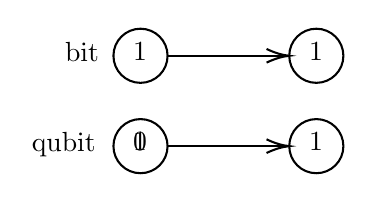
\begin{tikzpicture}[x=0.75pt,y=0.75pt,yscale=-1,xscale=1]
    %uncomment if require: \path (0,300); %set diagram left start at 0, and has height of 300
    % Text Node
    \draw    (117.29, 130) circle [x radius= 13.04, y radius= 13.04]   ;
    \draw (112.29,122) node [anchor=north west][inner sep=0.75pt]   [align=left] {1};
    % Text Node
    \draw    (202, 130) circle [x radius= 13.04, y radius= 13.04]   ;
    \draw (197,122) node [anchor=north west][inner sep=0.75pt]   [align=left] {1};
    % Text Node
    \draw    (202, 173.54) circle [x radius= 13.04, y radius= 13.04]   ;
    \draw (197,165.54) node [anchor=north west][inner sep=0.75pt]   [align=left] {1};
    % Text Node
    \draw (112.29,165.54) node [anchor=north west][inner sep=0.75pt]   [align=left] {0};
    % Text Node
    \draw    (117.29, 173.54) circle [x radius= 13.04, y radius= 13.04]   ;
    \draw (112.29,165.54) node [anchor=north west][inner sep=0.75pt]   [align=left] {1};
    % Text Node
    \draw (79.43,122) node [anchor=north west][inner sep=0.75pt]   [align=left] {bit};
    % Text Node
    \draw (63.43,165.54) node [anchor=north west][inner sep=0.75pt]   [align=left] {qubit};
    % Connection
    \draw    (130.32,173.54) -- (186.96,173.54) ;
    \draw [shift={(188.96,173.54)}, rotate = 180] [color={rgb, 255:red, 0; green, 0; blue, 0 }  ][line width=0.75]    (10.93,-3.29) .. controls (6.95,-1.4) and (3.31,-0.3) .. (0,0) .. controls (3.31,0.3) and (6.95,1.4) .. (10.93,3.29)   ;
    % Connection
    \draw    (130.32,130) -- (186.96,130) ;
    \draw [shift={(188.96,130)}, rotate = 180] [color={rgb, 255:red, 0; green, 0; blue, 0 }  ][line width=0.75]    (10.93,-3.29) .. controls (6.95,-1.4) and (3.31,-0.3) .. (0,0) .. controls (3.31,0.3) and (6.95,1.4) .. (10.93,3.29)   ;
    
    \end{tikzpicture}
    \caption{A comparison of measuring a single bit and a qubit. When measuring the bit, we get the same value that the bit is set to. When measuring a qubit, there is a certain probability of it being 0 and 1, so we measure one of both but don't know the real, internal state of the qubit.}
    \label{figure:comparison_bit_qubit_measurement}
\end{figure}

When measuring a quantum circuit, the qubit states collapse from super positions into the fixed position of 0 or 1. This means that to redo the measurement, the complete circuit has to be rebuilt. After doing multiple measurements on a qubit and collecting the results as shown in table \ref{table:example_counts}, this data can be used to construct a \emph{histogram}\cite{eckstein_lexikon_1994} akin to the one visualized in figure \ref{figure:example_histogram}, out of which one can retrieve the internal probabilities of 1 and 0.

\begin{figure}[!h]
    \begin{subtable}{.5\textwidth}
    \centering
    \begin{tabular}{|c|c|}
         Measured value & Amount  \\
         \hline
         0 & 547 \\
         1 & 987 \\
    \end{tabular}
    \caption{Table containing all measurements done on a qubit in an unknown superposition. The number of occurrences of a measured 1 or 0 is counted and then used to generate the histogram in figure \ref{figure:example_histogram}}
    \label{table:example_counts}
    \end{subtable}
    \begin{subfigure}{.5\textwidth}
        \centering
        \scalebox{\histogramwidth}{
            \includesvg{thesis/Appendices/example_histogram.svg}
        }
        \caption{A histogram generated from the data in table \ref{table:example_counts}, that visually shows the probabilities of 0 and 1. These probabilities can directly be used to understand the superposition of a qubit .}
        \label{figure:example_histogram}
    \end{subfigure}
    \caption{Example of collected measurements from an arbitrary, single qubit, quantum circuit, as well as the corresponding histogram.}
    \label{fig:my_label}
\end{figure}

With these two definitions, the gates used in the quantum circuits of this thesis can be fully 

\newpage

To further understand how a qubit behaves, the very foundations of quantum physics have to be looked at. Postulated by E. Schrödinger in 1925, the \emph{Schrödinger-Equation}\cite{PhysRev.28.1049} gives us the differential equation for the time evolution of a quantum state and their respective solution, shown in equation \ref{equation:schroedinger_time_evolution}, where $H$ denotes a Hamiltonian.

\begin{equation}
    \centering
    \begin{split}
        i\hbar\frac{d}{dt}\psi(t) =\ H\psi(t) \\
        \psi(t) =\ e^{-i\frac{Ht}{\hbar}}\psi(0)
    \end{split}
    \label{equation:schroedinger_time_evolution}
\end{equation}

The expression $U(t) =\ e^-i\frac{Ht}{\hbar}$ itself has the attribute that it is unitary. Through this, the multiplication of $U(t)$ with its conjugate transpose $U(t)^\ast$ results in the identity matrix. This leads to quantum operations being reversible – so-called \emph{bijective functions} - where every output can be reversed to a single input. \par
A mere two years later, Wolfgang Pauli published "Zur Quantenmechanik des magnetischen Elektrons"\cite{pauli_zur_1927}, in which he introduced the \emph{Pauli matrices}. These matrices represent the \emph{spin} of atoms and elementary particles, and are a core element of quantum computing. The definition of these matrices is shown in equation \ref{equation:pauli_matrices}.

\begin{equation}
    \centering
    \begin{split}
        \sigma_x &=\ \begin{pmatrix}0 & 1 \\ 1 & 0\end{pmatrix}\\
        \sigma_y &=\ \begin{pmatrix}0 & -i \\ i & 0\end{pmatrix}\\
        \sigma_z &=\ \begin{pmatrix}1 & 0 \\ 0 & -1\end{pmatrix}\\
    \end{split}
    \label{equation:pauli_matrices}
\end{equation}

\newpage

The \bloch\cite{michael_a_nielsen_quantum_2000}, as shown in figure \ref{figure:basic_bloch_sphere}, is used to help visualize quantum operations on a single, \emph{non-entangled}, qubit. The complex \emph{Bloch}-Vector inside the \bloch\ corresponds to the expectation value of measuring a value in a single qubit. To visualize entangled qubits, the \bloch\ by itself is not enough. There are proposed solutions to this problem\cite{gamel_entangled_2016}, which result in a more complex visualization with multiple \bloch s. To solve this issue, IBM created the Q-Sphere\cite{ibm_quantum_visualizations_nodate} as shown in figure \ref{figure:q_sphere_4qubit_h}, which can not only visualize single qubits, but also entangled ones as well as their global phase and probability in form of amplitude.

\begin{figure}[!h]
    \centering
    \begin{subfigure}{.4\textwidth}
        \centering
        \scalebox{\blochwidth}{
            \includesvg{thesis/Appendices/Bloch_Sphere_axis.svg}
        }
        \caption{A basic \bloch\ without any visualized state. The axis $x$ and $y$ are annotated accordingly, but the axis $z$ is annotated with $\ket{0}$ and $\ket{1}$ - the states which are measured and have a corresponding probability assigned to them. The purple arrow shows the \emph{Bloch}-Vector, and currently points to $\ket{0}$, so the state the single qubit is currently in.}
        \label{figure:basic_bloch_sphere}
    \end{subfigure}
    \begin{subfigure}{.5\textwidth}
        \centering
        \scalebox{\qspherewidth}{
            \includesvg{thesis/Appendices/Q_Sphere_State_h_multiqubit.svg}
        }
        \caption{A basic Q-Sphere that shows all possible states of a 4 qubit circuit, as well as the probability of each state, as well as their phase. The probability is encoded into the width of the dots next to the state labels. As all dots are equal, it is clear that all states have the same probability of being measured.}
        \label{figure:q_sphere_4qubit_h}
    \end{subfigure}
    \caption{A comparison of the \bloch\ used to visualize single qubits only, and the Q-Sphere that can visualize multiple qubits.}
    \label{fig:comparison_bloch_sphere_q_sphere}
\end{figure}

When measuring a qubit, the state collapses onto the $z$-axis\cite{feynman_feynman_1965}, which in turn leads to a measurement of either 0 or 1. Initially, all qubits are set to state $\ket{0}$, which is visualized onto the Q-Sphere in figure \ref{figure:state_0_q_sphere}. A circuit that results in said state is visualized in figure \ref{figure:state_0_circuit}, and its mathematical counterpart in equation \ref{equation:state_0_equation}. The states $\ket{\psi_i}$ are used to denote the state of one, or multiple, qubits at the currently marked point of the circuit. These are utilized to mark the states that are calculated throughout this thesis.

\begin{figure}[!h]
    \begin{subfigure}{.5\textwidth}
    \centering
        \scalebox{\qspherewidth}{
            \includesvg{thesis/Appendices/Q_Sphere_State_0.svg}
        }
        \caption{A Q-Sphere with the state $\ket{0}$ visualized onto it.}
        \label{figure:state_0_q_sphere}
    \end{subfigure}
    \begin{subfigure}{.5\textwidth}
    \centering
        \scalebox{1.0}{
        \Qcircuit @C=1.0em @R=1.0em @!R { \\
    	 	\nghost{{q} :  } & \lstick{{q} :  } \barrier[0em]{0} & \qw & \qw & \qw\\
    	 	\nghost{} & \lstick{} & \ket{\psi_0} &\\
    \\ }}
        \caption{A basic circuit consisting of a single qubit $q$ that is initially set to $\ket{0}$. The state vector at point $\ket{\psi_0}$ is shown in equation \ref{equation:state_0_equation}.}
        \label{figure:state_0_circuit}
    \end{subfigure}
    \caption{The circuit with qubit state $\ket{0}$ at position $\ket{\psi_0}$ and its corresponding Q-Sphere visualization.}
    \label{fig:showcase_qubit_state_0_with_circuit}
\end{figure}



\begin{equation}
    \centering
    \begin{split}
        \ket{\psi_0} =\ \begin{pmatrix}1 \\ 0\end{pmatrix} =\ \ket{0}\\
    \end{split}
    \label{equation:state_0_equation}
\end{equation}

\newpage
To create the state $\ket{1}$, the state of the qubit has to be turned by 180° around the $x$ or the $y$ axis. This can be achieved in multiple ways, but one simple way is using a \xgate\cite{qiskit_xgate_nodate}. A circuit with such a gate is visualized in figure \ref{figure:x_circuit}, with a \emph{Bloch}-Sphere visualization done in figure \ref{figure:state_1_bloch_sphere}.

\begin{figure}[!h]
    \centering
    \scalebox{\blochwidth}{
        \includesvg{thesis/Appendices/Bloch_Sphere_state_1.svg}
    }
    \caption{The \bloch with the state $\ket{1}$ visualized onto it, which was achieved through the usage of the circuit in figure \ref{figure:x_circuit}}
    \label{figure:state_1_bloch_sphere}
\end{figure}

\begin{figure}[!h]
    \centering\scalebox{1.0}{
    \Qcircuit @C=1.0em @R=0.2em @!R { \\
	 	\nghost{{q} :  } & \lstick{{q} :  } \barrier[0em]{0} & \qw & \gate{\mathrm{X}} \barrier[0em]{0} & \qw & \qw & \qw\\
	 	\nghost{} & \lstick{} & \ket{\psi_0} & & \ket{\psi_1} &\\
\\ }}
    \caption{A simple circuit with one qubit, that is transformed through the usage of a \xgate\ to transform the initial state $\ket{0}$, which the qubit $q$ has at position $\ket{\psi_0}$, into the state $\ket{1}$ at position $\ket{\psi_1}$}
    \label{figure:x_circuit}
\end{figure}

\begin{equation}
    \centering
    \begin{split}
        \ket{\psi_1} =\ \mathrm{X}\ket{\psi_0} =\ \begin{pmatrix} 0 & 1\\ 1 & 0\end{pmatrix}\begin{pmatrix}1 \\ 0\end{pmatrix} =\ \begin{pmatrix}0 \\ 1 \end{pmatrix}\\
    \end{split}
    \label{equation:state_1_equation}
\end{equation}

The state $\ket{\psi_1}$ is directly calculated, as demonstrated in equation \ref{equation:state_1_equation}. The same can be done with the gates \ygate\cite{qiskit_ygate_nodate} and \zgate\cite{qiskit_zgate_nodate} that apply a full 180° rotation around their corresponding axes. \par
The \emph{Hadamard}-Gate, or \hgate\cite{qiskit_hgate_nodate}, can be used to quickly create a superposition of a single qubit where the state $\ket{0}$ and $\ket{1}$ have the same probability (exactly 0.5) of being measured. Without it, one would have to use a combination of different gates to achieve the result\cite{voorhoede_hadamard_nodate}, for example $\mathrm{XY}^{\frac{1}{2}}$.

\begin{figure}[!h]
    \centering\scalebox{1.0}{
    \Qcircuit @C=1.0em @R=0.2em @!R { \\
	 	\nghost{{q} :  } & \lstick{{q} :  } \barrier[0em]{0} & \qw & \gate{\mathrm{H}} \barrier[0em]{0} & \qw & \qw & \qw\\
	 	\nghost{} & \lstick{} & \ket{\psi_0} & & \ket{\psi_1} &\\
\\ }}
    \caption{A simple circuit with one qubit, that is transformed
through the usage of a \hgate\ to turn the initial state $\ket{0}$ at position $\ket{\psi_0}$, which into the state $\ket{1}$ at position $\ket{\psi_1}$.}
    \label{figure:h_circuit}
\end{figure}

\begin{equation}
    \centering
    \begin{split}
        \ket{\psi_1} =\ \mathrm{H}\ket{\psi_0} =\ \frac{1}{\sqrt{2}}\begin{pmatrix} 1 & 1 \\ 1 & -1 \end{pmatrix}\begin{pmatrix}1 \\ 0\end{pmatrix} =\ \frac{1}{\sqrt{2}}\begin{pmatrix}1 \\ 0 \end{pmatrix} + \frac{1}{\sqrt{2}}\begin{pmatrix}0 \\ 1 \end{pmatrix}\\
    \end{split}
    \label{equation:equal_superposition_equation}
\end{equation}

\begin{figure}[!h]
    \centering
    \scalebox{\blochwidth}{
        \includesvg{thesis/Appendices/Bloch_Sphere_state_0_1_equal.svg}
    }
    \caption{A basic \emph{Bloch}-Sphere with the state $\frac{1}{\sqrt{2}}\begin{pmatrix}1 \\ 0 \end{pmatrix} + \frac{1}{\sqrt{2}}\begin{pmatrix}0 \\ 1 \end{pmatrix}$ visualized onto it.}
    \label{figure:state_h_bloch_sphere}
\end{figure}

To assess that the visualization, and the described behaviour of qubits is correct, these assumptions can be evaluated the formal way. When calculating the to be expected probability of a certain state, the Hermitian transposition\cite{marshall_c_methods_1964} is used. Equation \ref{equation:basic_h_measurement} demonstrates the calculation of the probabilities the \hgate\ assigns to the measurements of $0$ and $1$.

\begin{equation}
    \centering
    \begin{split}
        \ket{\psi_1} &=\ \frac{1}{\sqrt{2}}\ket{0} + \frac{1}{\sqrt{2}}\ket{1}\\
        \bra{0}\ket{\psi_1} &=\ \frac{1}{\sqrt{2}}\begin{pmatrix}1 & 0 \end{pmatrix}\begin{pmatrix}1 \\ 0 \end{pmatrix} + \frac{1}{\sqrt{2}}\begin{pmatrix}1 & 0 \end{pmatrix}\begin{pmatrix}0 \\ 1 \end{pmatrix} \\
        \bra{0}\ket{\psi_1} &=\ \frac{1}{\sqrt{2}}\\
        |\bra{0}\ket{\psi_1}|^2 &=\ 0.5\\
        |\bra{1}\ket{\psi_1}|^2 &=\ \left|\frac{1}{\sqrt{2}}\right|^2 =\ 0.5\\
    \end{split}
    \label{equation:basic_h_measurement}
\end{equation}

As shown, both states $\ket{0}$ and $\ket{1}$ have the same probability of $0.5$. When desiring probabilities that are not equal for both states, there are gates the likes of \rygate\cite{qiskit_rygate_nodate}, \rxgate\cite{qiskit_rxgate_nodate} and \rzgate\cite{qiskit_rzgate_nodate}. These gates allow the rotation around the corresponding axes by a given parameter. To create a circuit that achieves the probabilities from the histogram, \ref{figure:example_histogram}, these gates are needed. Equation \ref{equation:rx_gate_definition} shows the definition of the \rygate.

\begin{equation}
    \centering
    \begin{split}
        \mathrm{RY}(\theta) =\ \begin{pmatrix} \cos{\frac{\theta}{2}}   & -\sin{\frac{\theta}{2}} \\
        -\sin{\frac{\theta}{2}} & \cos{\frac{\theta}{2}}
    \end{pmatrix}
    \end{split}
    \label{equation:rx_gate_definition}
\end{equation}

The formal definition used in equation \ref{equation:basic_h_measurement} as well as the \rygate\ can be combined to calculate the parameters needed to achieve the probabilities shown in \ref{figure:example_histogram}, as demonstrated in equation \ref{equation:parameter_from_probabilities}. 

\begin{equation}
    \centering
    \begin{split}
        |\bra{1}\ket{\psi_1}|^2 &=\ 0.643 \\
        \begin{pmatrix}1 & 0\end{pmatrix}\ket{\psi_1} &=\ \sqrt{0.643} \\
        \ket{\psi_1} &=\ \sqrt{0.357}\begin{pmatrix} 1 \\ 0\end{pmatrix} + \sqrt{0.643}\begin{pmatrix} 0 \\ 1\end{pmatrix}\\
        \ket{\psi_1} &=\ \begin{pmatrix}\sqrt{0.643}\\ \sqrt{0.357}\end{pmatrix}\\
        \mathrm{RY}(\theta)\ket{0} &=\ \begin{pmatrix}\sqrt{0.357}\\ \sqrt{0.643}\end{pmatrix} \\
        \begin{pmatrix}\cos{\frac{\theta}{2}} \\ -i\sin{\frac{\theta}{2}}\end{pmatrix} &=\ \begin{pmatrix}\sqrt{0.357}\\ \sqrt{0.643}\end{pmatrix}\\
        \theta_{cos} &=\ 2(\acos{\sqrt{0.357}}) =\ 1.8608\\
        \theta_{sin} &=\ 2(\asin{\sqrt{0.643}}) =\ 1.8608\\
        \theta &=\ \theta_{sin} =\ \theta_{cos}\\
    \end{split}
    \label{equation:parameter_from_probabilities}
\end{equation}

With the value for $\theta$ calculated, the circuit from figure \ref{figure:circuit_for_histogram} is designed and evaluated to compare it to the histogram from \ref{figure:example_histogram} to the one in figure \ref{figure:circuit_histogram}.

\begin{figure}[!h]
    \centering
    \scalebox{1.0}{
    \Qcircuit @C=1.0em @R=0.2em @!R { \\
    	 	\nghost{{q} :  } & \lstick{{q} :  } & \gate{\mathrm{R_Y}\,(\mathrm{1.8608})} & \qw & \qw\\
    \\ }}
    \caption{A circuit designed with a parameterized \rygate, that allows the usage of the calculated value $1.8608$ to generate the histogram \ref{figure:circuit_histogram}, which equals the example histogram from \ref{figure:example_histogram}}
    \label{figure:circuit_for_histogram}
\end{figure}


\begin{figure}[!h]
    \centering
    \scalebox{\histogramwidth}{
        \includesvg{thesis/Appendices/calculated_circuit_histogram.svg}
    }
    \caption{A histogram generated from the data in table \ref{table:example_counts}, that visually shows the probabilities of 0 and 1. These probabilities can directly be used to visualize the qubits superposition.}
    \label{figure:circuit_histogram}
\end{figure}

%%%%%%%%%%%%%%%%%%%%%%%%%%%%%%%%%%%%%%

\newpage

\section{Multiple Query Optimization}

A query\cite{codd_relational_1970} is a demand for information to be pulled from a database. Such a query can vary in size and structure, as well as in execution time. These are often written in the query language \code{SQL}, which is often adapted to the corresponding software\cite{shirgoldbird_microsoft_nodate}\cite{the_postgresql_global_development_group_postgresql_2022} it executes on. 

    
\begin{figure}[!h]
    \centering
    \begin{minted}{sql}
        SELECT * FROM USERS u
        WHERE u.NAME = "Abraham"
    \end{minted}
    \caption{This example SQL code would tell the database we want all data from table \emph{USER}, where the name equals \emph{Abraham}}
    \label{figure:sql_query_example}
\end{figure}

The example query in figure \ref{figure:sql_query_example} is parsed, and the resulting query plan used to retrieve and display data that is saved in the database. Table \ref{table:sql_query_result_example} resembles the result of such a query.

\begin{table}[!h]
    \centering
    \begin{tabular}{|c|c|c|}
        \hline
        Name    & Surname & Gender \\ \hline
        Abraham & Martin  & M      \\ \hline
        Abraham & Tart    & F      \\ \hline
    \end{tabular}
    \caption{Exemplary data returned after executing the SQL query from figure \ref{figure:sql_query_example}, where the first row resembles the name of the attributes in the column}
    \label{table:sql_query_result_example}
\end{table}

Before any execution takes place, the queries themselves are parsed into multiple execution plans\cite{microsoft_execution_nodate}. These plans usually resemble the same operations, just in a different order – this can result in precious time savings. In a large system that handles multiple requests per second, these plans can be used to combine certain sub-sequences of a plan and therefore save execution time\cite{roy_multi-query_2009}. This by itself has been proven to be an \emph{NP-Hard} problem\cite{sellis_multiple-query_1990}. Nevertheless, finding the fastest combination of all plans can be done classically with an exhaustive algorithm in $O(P^Q)$\footnote{as long as all queries have the same number of plans}, where $P$ is the number of plans and $Q$ the number of queries. The work of Kathurina et al.\cite{kathuria_provable_mqo} offers a greedy algorithm for finding a \emph{good} solution, whilst also proving that finding a better approximation factor for the greedy algorithm is \emph{NP-Hard}. A hybrid approach that combines classical and quantum computing uses QAOA (short for Quantum Approximate Optimization Algorithm)\cite{farhi_quantum_2014} have shown to be quasi-optimal solution finders with a runtime of $O(I \cdot (PQ)^2)$\cite{fankhauser_multiple_2021}. \par

\subsection{Query Dissection}
A query can be dissected into a variety of plans that can be executed to get the data in the desired format. Figure \ref{figure:query_with_plans} shows a query, which has two differing plans.

\begin{figure}[!h]
    \centering
    \tikzset{every picture/.style={line width=0.75pt}} %set default line width to 0.75pt        
    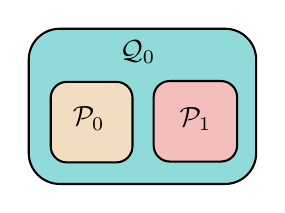
\begin{tikzpicture}[x=0.75pt,y=0.75pt,yscale=-1,xscale=1]
        %uncomment if require: \path (0,300); %set diagram left start at 0, and has height of 300
        %Rounded Rect [id:dp08144411333317714] 
        \draw  [fill={rgb, 255:red, 144; green, 218; blue, 217 }  ,fill opacity=1 ] (80.2,130.56) .. controls (80.2,122.3) and (86.9,115.6) .. (95.16,115.6) -- (174.84,115.6) .. controls (183.1,115.6) and (189.8,122.3) .. (189.8,130.56) -- (189.8,175.44) .. controls (189.8,183.7) and (183.1,190.4) .. (174.84,190.4) -- (95.16,190.4) .. controls (86.9,190.4) and (80.2,183.7) .. (80.2,175.44) -- cycle ;
        %Rounded Rect [id:dp5870651506756062] 
        \draw  [fill={rgb, 255:red, 242; green, 221; blue, 192 }  ,fill opacity=1 ] (90.8,148.96) .. controls (90.8,144.67) and (94.27,141.2) .. (98.56,141.2) -- (122.44,141.2) .. controls (126.73,141.2) and (130.2,144.67) .. (130.2,148.96) -- (130.2,172.24) .. controls (130.2,176.53) and (126.73,180) .. (122.44,180) -- (98.56,180) .. controls (94.27,180) and (90.8,176.53) .. (90.8,172.24) -- cycle ;
        %Rounded Rect [id:dp7624346816043626] 
        \draw  [fill={rgb, 255:red, 243; green, 190; blue, 188 }  ,fill opacity=1 ] (140.4,148.56) .. controls (140.4,144.27) and (143.87,140.8) .. (148.16,140.8) -- (172.84,140.8) .. controls (177.13,140.8) and (180.6,144.27) .. (180.6,148.56) -- (180.6,171.84) .. controls (180.6,176.13) and (177.13,179.6) .. (172.84,179.6) -- (148.16,179.6) .. controls (143.87,179.6) and (140.4,176.13) .. (140.4,171.84) -- cycle ;
        % Text Node
        \draw (151.4,152.2) node [anchor=north west][inner sep=0.75pt]   [align=left] {$\displaystyle \mathcal{P}_{1}$};
        % Text Node
        \draw (100,151.8) node [anchor=north west][inner sep=0.75pt]   [align=left] {$\displaystyle \mathcal{P}_{0}$};
        % Text Node
        \draw (122.8,119.8) node [anchor=north west][inner sep=0.75pt]   [align=left] {$\displaystyle \mathcal{Q}_{0}$};
    \end{tikzpicture}
    \caption{A query that can be executed through two different plans, which end up delivering the same result but might offer potential time savings.}
    \label{figure:query_with_plans}
\end{figure}

The plans themselves consist of many different instructions, which can be as simple as loading a table from storage into memory or searching a certain table for a given value. If one were to add another query that is to be executed parallel to the one in figure \ref{figure:query_with_plans}, overlapping instructions could be combined so that they're executed exactly once, and then reused for both plans, as shown in figure \ref{figure:plan_tree}. Each instruction in any plan consist of single operations applied to tables of the database that are based on relational algebra\cite{codd_relational_1970}\footnote{But not limited to them, as modern databases also include hashing and indexing in the plans. None the less, these operations can also be combined to save previous runtime}. It is easy to imagine that, depending on the environment at hand, single operations will happen plenty of times in parallel. Putting into perspective the number of users that modern applications\cite{uber_technologies_inc_uber_2022} can have, finding shortcuts in plans does not only reduce execution time but saves money and improves customer experience.

\begin{figure}[!h]
    \centering
\tikzset{every picture/.style={line width=0.75pt}} %set default line width to 0.75pt        

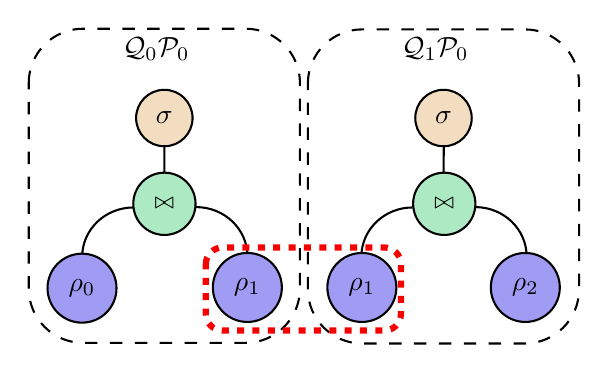
\begin{tikzpicture}[x=0.75pt,y=0.75pt,yscale=-1,xscale=1]
%uncomment if require: \path (0,300); %set diagram left start at 0, and has height of 300

%Rounded Rect [id:dp3098689700784747] 
\draw  [dash pattern={on 4.5pt off 4.5pt}] (120.33,155.05) .. controls (120.33,140.62) and (132.03,128.92) .. (146.47,128.92) -- (224.87,128.92) .. controls (239.3,128.92) and (251,140.62) .. (251,155.05) -- (251,254.12) .. controls (251,268.55) and (239.3,280.25) .. (224.87,280.25) -- (146.47,280.25) .. controls (132.03,280.25) and (120.33,268.55) .. (120.33,254.12) -- cycle ;
%Shape: Arc [id:dp8469571253916317] 
\draw  [draw opacity=0] (146.09,238.65) .. controls (146.2,225.59) and (157.23,215.04) .. (170.82,215.04) -- (170.82,238.86) -- cycle ; \draw   (146.09,238.65) .. controls (146.2,225.59) and (157.23,215.04) .. (170.82,215.04) ;  
%Shape: Arc [id:dp8173590455021038] 
\draw  [draw opacity=0] (201,214.86) .. controls (214.66,214.86) and (225.73,225.52) .. (225.73,238.67) -- (201,238.67) -- cycle ; \draw   (201,214.86) .. controls (214.66,214.86) and (225.73,225.52) .. (225.73,238.67) ;  
%Straight Lines [id:da6630213040029864] 
\draw    (185.68,199.4) -- (185.67,186) ;
%Rounded Rect [id:dp5436966787626745] 
\draw  [dash pattern={on 4.5pt off 4.5pt}] (254.83,155.38) .. controls (254.83,140.95) and (266.53,129.25) .. (280.97,129.25) -- (359.37,129.25) .. controls (373.8,129.25) and (385.5,140.95) .. (385.5,155.38) -- (385.5,254.45) .. controls (385.5,268.88) and (373.8,280.58) .. (359.37,280.58) -- (280.97,280.58) .. controls (266.53,280.58) and (254.83,268.88) .. (254.83,254.45) -- cycle ;
%Shape: Arc [id:dp13654717695684715] 
\draw  [draw opacity=0] (280.59,238.65) .. controls (280.7,225.59) and (291.73,215.04) .. (305.32,215.04) -- (305.32,238.86) -- cycle ; \draw   (280.59,238.65) .. controls (280.7,225.59) and (291.73,215.04) .. (305.32,215.04) ;  
%Shape: Arc [id:dp7676498647138272] 
\draw  [draw opacity=0] (335.5,214.86) .. controls (349.16,214.86) and (360.23,225.52) .. (360.23,238.67) -- (335.5,238.67) -- cycle ; \draw   (335.5,214.86) .. controls (349.16,214.86) and (360.23,225.52) .. (360.23,238.67) ;  
%Straight Lines [id:da7192788563309687] 
\draw    (320.18,199.4) -- (320.33,184.44) ;
%Rounded Rect [id:dp6770297453454031] 
\draw  [color={rgb, 255:red, 246; green, 1; blue, 1 }  ,draw opacity=1 ][dash pattern={on 2.53pt off 3.02pt}][line width=2.25]  (205.67,242.33) .. controls (205.67,237.92) and (209.25,234.33) .. (213.67,234.33) -- (291.67,234.33) .. controls (296.08,234.33) and (299.67,237.92) .. (299.67,242.33) -- (299.67,266.33) .. controls (299.67,270.75) and (296.08,274.33) .. (291.67,274.33) -- (213.67,274.33) .. controls (209.25,274.33) and (205.67,270.75) .. (205.67,266.33) -- cycle ;

% Text Node
\draw (164.17,131.65) node [anchor=north west][inner sep=0.75pt]    {$\mathcal{Q}_{0}\mathcal{P}_{0}$};
% Text Node
\draw  [fill={rgb, 255:red, 242; green, 221; blue, 192 }  ,fill opacity=1 ]  (185.67, 171.95) circle [x radius= 13.6, y radius= 13.6]   ;
\draw (185.67,171.95) node    {$\sigma $};
% Text Node
\draw (298.67,131.65) node [anchor=north west][inner sep=0.75pt]    {$\mathcal{Q}_{1}\mathcal{P}_{0}$};
% Text Node
\draw  [fill={rgb, 255:red, 242; green, 221; blue, 192 }  ,fill opacity=1 ]  (320.17, 171.95) circle [x radius= 13.6, y radius= 13.6]   ;
\draw (320.17,171.95) node    {$\sigma $};
% Text Node
\draw  [fill={rgb, 255:red, 173; green, 234; blue, 195 }  ,fill opacity=1 ]  (185.71, 213.28) circle [x radius= 15, y radius= 15]   ;
\draw (185.71,213.28) node  [font=\footnotesize]  {$\bowtie $};
% Text Node
\draw  [fill={rgb, 255:red, 173; green, 234; blue, 195 }  ,fill opacity=1 ]  (320.54, 213.28) circle [x radius= 15, y radius= 15]   ;
\draw (320.54,213.28) node  [font=\footnotesize]  {$\bowtie $};
% Text Node
\draw  [fill={rgb, 255:red, 160; green, 156; blue, 243 }  ,fill opacity=1 ]  (146.01, 253.92) circle [x radius= 16.62, y radius= 16.62]   ;
\draw (146.01,253.92) node   [align=left] {$\displaystyle \rho _{0}$};
% Text Node
\draw  [fill={rgb, 255:red, 160; green, 156; blue, 243 }  ,fill opacity=1 ]  (225.67, 253.58) circle [x radius= 16.62, y radius= 16.62]   ;
\draw (225.67,253.58) node   [align=left] {$\displaystyle \rho _{1}$};
% Text Node
\draw  [fill={rgb, 255:red, 160; green, 156; blue, 243 }  ,fill opacity=1 ]  (280.84, 253.58) circle [x radius= 16.62, y radius= 16.62]   ;
\draw (280.84,253.58) node   [align=left] {$\displaystyle \rho _{1}$};
% Text Node
\draw  [fill={rgb, 255:red, 160; green, 156; blue, 243 }  ,fill opacity=1 ]  (359.59, 253.58) circle [x radius= 16.62, y radius= 16.62]   ;
\draw (359.59,253.58) node   [align=left] {$\displaystyle \rho _{2}$};


\end{tikzpicture}


    \caption{Two differing plans $\mathcal{Q}_0\mathcal{P}_0$ and $\mathcal{Q}_1\mathcal{P}_1$, which serve different goals but contain the same operation $\rho_1$, marked in the red dotted box}
    \label{figure:plan_tree}
\end{figure}

Figure \ref{figure:plan_tree} shows two different queries that contain the same sub-operation $\rho_1$. The operation can be used by both queries, which means we do not have to execute it twice. This example would be one of the most common forms of saving execution time: \emph{Loading the data once and then re-using it during evaluation}.

Plans, costs, and savings can be mathematically expressed. Let there be given function $\mathcal{C}$ which returns the cost for a given operation or collection of operations, as defined in equation \ref{equation:formal_cost_function}. Let there also be a given function $\mathcal{S}$, which calculates the savings two collections of operations can achieve, as shown in equation \ref{equation:formal_savings_function}.

\begin{equation}
    \centering
    \begin{split}
        \mathcal{C}(\mathcal{Q}_0\mathcal{P}_1) =\ 45 \\
        \mathcal{C}(\rho_1) =\ 15 \\
    \end{split}
    \label{equation:formal_cost_function}
\end{equation}

\begin{equation}
    \centering
    \begin{split}
        \mathcal{S}(\mathcal{Q}_0\mathcal{P}_1, \mathcal{Q}_1\mathcal{P}_0) =\ 15 \\
        \mathcal{S}(\mathcal{Q}_0\mathcal{P}_0, \mathcal{Q}_1\mathcal{P}_1) =\ 0 \\
    \end{split}
    \label{equation:formal_savings_function}
\end{equation}


Taking a problem consisting of two queries $\mathcal{Q}_0$ and $\mathcal{Q}_1$, each of which has two plans $\mathcal{P}_0$ and $\mathcal{P}_1$, we can calculate the total costs of running them collectively as shown in equation \ref{equation:formal_total_cost_calculation}.

\begin{equation}
    \centering
    \begin{split}
        \mathcal{C}(\mathcal{Q}_0\mathcal{P}_0) + \mathcal{C}(\mathcal{Q}_1\mathcal{P}_0) - \mathcal{S}(\mathcal{Q}_0\mathcal{P}_0, \mathcal{Q}_1\mathcal{P}_0) \\
        \mathcal{C}(\mathcal{Q}_0\mathcal{P}_0) + \mathcal{C}(\mathcal{Q}_1\mathcal{P}_1) - \mathcal{S}(\mathcal{Q}_0\mathcal{P}_0, \mathcal{Q}_1\mathcal{P}_1) \\
        \mathcal{C}(\mathcal{Q}_0\mathcal{P}_1) + \mathcal{C}(\mathcal{Q}_1\mathcal{P}_0) - \mathcal{S}(\mathcal{Q}_0\mathcal{P}_1, \mathcal{Q}_1\mathcal{P}_0) \\
        \mathcal{C}(\mathcal{Q}_0\mathcal{P}_1) + \mathcal{C}(\mathcal{Q}_1\mathcal{P}_1) - \mathcal{S}(\mathcal{Q}_0\mathcal{P}_1, \mathcal{Q}_1\mathcal{P}_1) \\
    \end{split}
    \label{equation:formal_total_cost_calculation}
\end{equation}

If we change the problem space from two queries to more, or create an uneven number of plans per query, the complexity starts to rise sharply.


%%%%%%%%%%%%%%%%%%%%%%%%%%%%%%%%%%%%%%

\newpage

\section{Quantum Neural Network}

\subsection{Quantum Neural Network}


\subsection{Quantum Support Vector Machine (SVM)}
A classical support vector machine (SVM) also known as support vector network, initially conceived of by Cortes and Vapnik, divides a set of objects into classes in such a way that the widest possible area around the class boundaries remains free of objects. SVMs can not only perform linear classifications but also non-linear ones using the so-called kernel trick \cite{Cortes2004SupportVectorN}. A detailed explanation on how classical Support Vector Machines work can be found in the paper “Support vector machines explained” by Tristan Fletcher \cite{fletcher2009support}. 

Quantum SVM is considered to be the quantum analogue of the classical SVM algorithm as stated by Jiaying Yang et al. \cite{yangSupportVectorMachines2019}.

